\documentclass{article}
\usepackage{amsmath,amssymb}
\usepackage{graphicx}
\usepackage[top=3cm, bottom=3cm, right=3cm, left=3cm]{geometry}
\usepackage{hyperref}
\hypersetup{
    colorlinks,
    citecolor=black,
    filecolor=black,
    linkcolor=black,
    urlcolor=black
}


\begin{document}

\newpage{}
\tableofcontents
\newpage{}

\newpage
\section{Teoria de Colas}

\subsection{Introducción}
\subsubsection{Conceptos basicos}

Los fenónmenos de \textit{congestión} o \textit{espera} estan relacionados con los sistemas estocasticos y pueden describirse como sistemas integrados por uno o mas \textit{centros de atención} donde se brinda un servicio.
Cada centro de atención es, a su vez, un sistema constituido por:

\begin{itemize}
    \item \textit{canales (ó servidores)}: Entidades que prestan el servicio. 
    \item \textit{clientes (ó usuario)}: Entidades que reciben el servicio. 
\end{itemize}

    \begin{figure}[h!]
        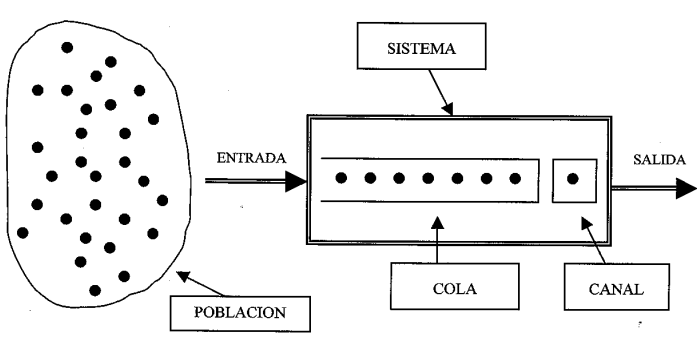
\includegraphics[width=0.8\textwidth]{imagenes/modelo_sistema.png}
    \end{figure}

Las colas se forman cuando la demande de un servicio dado en un intervalo de tiempo exede la capacidad para proveerlo.
El administrador del sistema de establecer un balance apropiado entre los costos asociados a la espera de los usuarios y los costos vinculados con la mejora del servicio (mas servidores, mayor velocidad de atención, etc).
En la mayoria de los procesos de atención, los tiempos entre arribos de clientes y los tiempos de los servicios no son predecibles. En estas condiciones se aplica la denomida \textit{teoría de colas} para determinar el comportamiento del sistema bajo diferentes alternativas.
Se estudiaran aquellos sistemas que describan los procesos mas generales y que son los que pueden formularse como \textit{cadenas markovianas de primer orden}. Se analisaran los sistemas en regimen permanente, a través de variables tales como la \textit{longitud promedio de la cola}, el \textit{tiempo de espera promedio} del cliente para recibir el servicio, el \textit{tiempo de permanencia} en el sistema, etc. 
Esta información, junstamente con los costos relevantes, permitira al directivo determinar los valores apropiados de las variables de decisión. Las variables de decisión tipicas en los sistemas de colas estan referidas a la \textit{capacidad de servicio}(numero de canales, velocidad de canales) ó la \textit{capadidad de espera} (número de lugares).

    \begin{figure}[h!]
        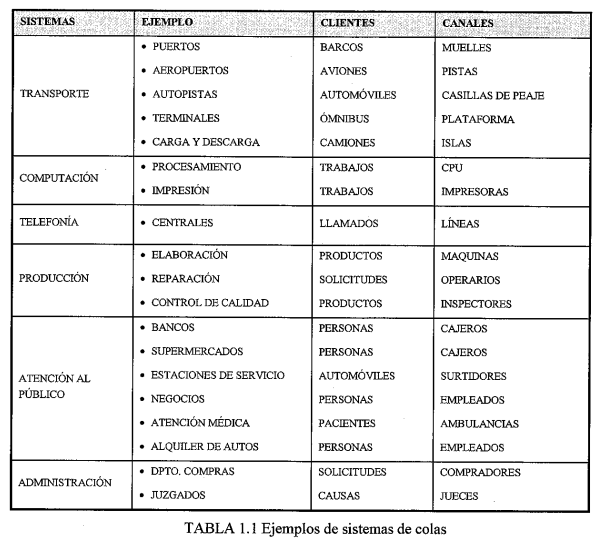
\includegraphics[width=\linewidth]{imagenes/ejemplo_sistemas_colas.png}
    \end{figure}

La \textbf{población} es el conjunto de usuario potenciales del sistema. Puede ser finito o infini  to.

En los \textbf{arribos} la llegada de los clientes puede ser deterministica o aleatoria. A menudo los intervalos entre llegadas son estadisticamente independientes y estacionarios a lo largo de prolongados periodos de tiempo, por lo que se puede suponer poissonianos.

La \textbf{impaciencia} se verifica cuando algunos usuarios que arriban al sistema se retiran sin recibir el servicio porque consideran que el tiempo de espera sera suficientemente largo. Se distingen dos tiempos de impaciencia:
\begin{enumerate}
    \item \textbf{Rechazo ($\overline{R}$)}: Un cliente que arriba, observa la cantidad de gente que esta delante de él esperando y en función de ello toma la decisión de incorporarse o no al sistema. \textbf{En la materia se trata unicamente este tipo de impaciencia}.
    \item \textbf{Abandono ($\overline{A}$)}: Un cliente que arriba, ingresa al sistema y al cabo de un tiempo toma la decisión de seguir esperando o no.
\end{enumerate}

La \textbf{capacidad} es el número máximo de clientes que puede permanecer en el sistema simultaneamente(en espera y atendiéndose).

Para el \textbf{modo de arribo} los usuarios pueden llegar en forma individual o en masa(modo batch). En la mayoria de los sistemas que estudiaremos se hará la suposición de que los procesos de llegado son del tipo Poisson, lo que implica \textit{arribos individuales}. Se puede considerar el arribo de grupos como clientes individuales. 

Para la \textbf{prioridad de atención}, existen diversos criterios de atención en lo que se refiere al orden de selección de clientes para brindar el servicio. Ellos son:

\begin{itemize}
    \item \underline{Base FIFO{(first in, first out)}}: Los clientes se atienden según el orden de llegada.
    \item \underline{Base LIFO{(last in, first out)}}: El último individuo que arriba es el primero en ser atendido.
    \item \underline{Base SIRO\textit{(service in random order)}}: Es una selección aleatoria de los clientes para brindales el servicio. 
    \item \underline{Base con PRIORIDADES}: Se establecen criterios de atención conforme a los atributos de los clientes. 
\end{itemize}

La \textbf{duración del servicio} es el tiempo requerido por un canal para atender un cliente. Puede ser una variable deterministica o aleatoria con distribución de probabilidad conocida.

En el \textbf{modo de atención} un canal puede servicio de forma individual o multiples(en masa). En la mayoria de los sistemas reales, el modo de atención es individual.

Los \textbf{procesos poisson} son markovianos y tienen dos distribuciones que lo describen:
\begin{enumerate}
    \item La distribución Poisson, en donde la variable es el número de eventos que se producen en un intervalo determinado de continuo.
    \item La distribución Gamma, en la que la variable es el intervalo de continuo necesario para que se verifique un número determinado de eventos. Partucularmente, cuando la variable es el intervalo de tiempo de continuo necesario para que se verifique \textit{un solo evento}, la distribución es conocida como \textbf{distribución Exponencial}. 
\end{enumerate}

\underline{Distribución Poisson}
La probabilidad de que se produzcan "n" eventos en un intervalo "t" estada dada por:
\begin{equation}
    p(n)= \frac{( \lambda \Delta t) ^ { n } \cdot e^{ - \lambda \Delta t}}{n!}
\end{equation}
siendo \(n=1,2,...\) y \( \lambda > 0\)
La media de esta distribución es \(a = \lambda . t\) y el desvio estandar \(\sigma=\sqrt{\lambda t}\).

\underline{Distribución Gamma}
La función distribución de probabilidad de la \textbf{distribución exponencial} esta dada por la siguiente expresión:

\begin{equation}
    f(t) = \lambda . e^{-\lambda t}
\end{equation}
cuya media es \(\frac{1}{\lambda}\)
y cuyo desvio estandar es \(\frac{1}{\lambda}\)

Si el proceso de arribos es de tipo Poisson significa que la variable "tiempo entre dos arribos sucesivos" tiene distribución \textit{exponencial} y la variable "numero de clientes que arriban por unidad de tiempo" tiene distribución \textit{Poisson}.

\textbf{Ingresos y egresos de clientes}: 
En los sistemas de capacidad finita o de población impaciente, no todos los clientes que arriban al sistema ingresan.
\begin{itemize}
    \item $\overline{\lambda}$: Número promedio de clientes que ingresan efectivamente al sistema.
    \item $\overline{R}$: Número promedio de rechazados(es decir, que no ingresan al sistema).
    \item $\overline{\mu}$: Número promedio de clientes atendidos que egresan del sistema.
    \item $\overline{A}$: Tasa de clientes que ingresaron al sistema pero que decidieron abandonarlo sin recibir el servicio.
\end{itemize}


\newpage
\textbf{Estructuras de sistemas simples}:
\begin{figure}[h!]
    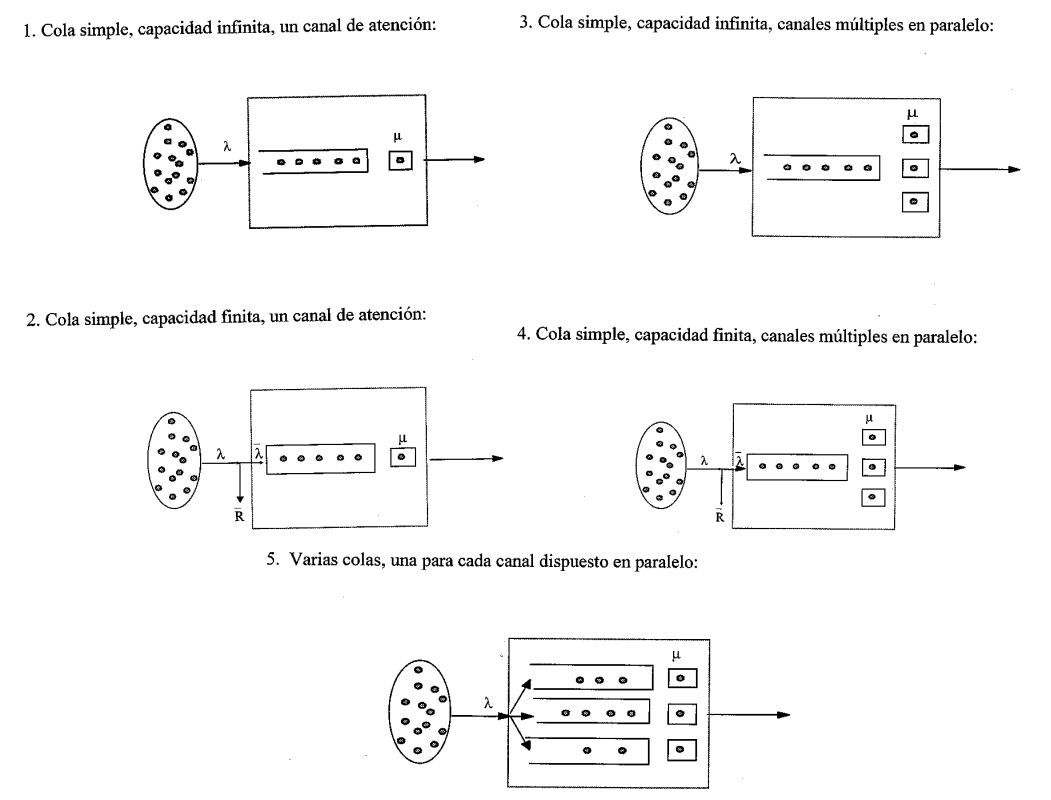
\includegraphics[width=\linewidth]{imagenes/estructuras_simples.png}
\end{figure}

\newpage
\subsubsection{Notación Kendall}
Especifica las caracteristicas descriptivas de una unidad operativa de un sistema de colas. Es una notación de 6 posiciones:
\begin{equation}
    1 / 2 / 3 / 4 / 5 / 6    
\end{equation}

\begin{enumerate}
    \item La posición 1 se refiere al patrón de arribos al sistema. Puede ser:
    \begin{itemize}
        \item P: Proceso de Poisson.
        \item D: Proceso deterministico.
        \item G: Cualquier otro proceso.
    \end{itemize}
    \item La posición 2 indica el patrón de servicio en los canales.
    \begin{itemize}
        \item P: Proceso de Poisson.
        \item D: Proceso deterministico.
        \item G: Cualquier otro proceso.
    \end{itemize}
    \item La posición 3 indica el número de canales de atención dispuestos en paralelo en la unidad operativa.
    \item La posición 4 indica la capacidad de la unidad operativa del sistema(Los que pueden esperar en la cola mas los que se pueden atender). Se asume infinita y no se indica.
    \item La posición 5 indica la prioridad de atension de la cola.  Si no se especifica se asume de tipo FIFO.
    \begin{itemize}
        \item FIFO
        \item LIFO
        \item SIRO
        \item G: Cualquier otra modalidad de atención
    \end{itemize}
    \item La última posición (entre paréntesis) se refiere al tamaño de la población. Si no se indica, el tamaño es infinito.
\end{enumerate}


\subsubsection{Ecuacion de estado de regimen permante}

Cuando el valor de las variables depende de las condiciones iniciales en las que se encontraba el sistema
cuando comenzo el proceso de observación, se dice que el sistema esta en \textbf{régimen transitorio}.

Si al transcurrir el tiempo, las variables se estabilizan y ya no dependen del estado inicial. Se dice que
a partir de ese momento, el sistema alcanza el \textbf{regimen permanente (o estacionario)}

\begin{equation}
    0 = p(n-1) \cdot \lambda_{n-1} - p(n) \cdot [\lambda_n + \mu_n] + p(n+1) \cdot \mu_{n+1}
\end{equation}


\subsubsection{Ecuacion simplificada de estado de regimen permante}

\begin{equation}
    p(n)= p(n-1) \cdot \frac{ \lambda_{n-1}}{\mu_n}
\end{equation}



\newpage
\subsubsection{Preguntas y respuestas}
\begin{itemize}
    \item ¿Qué características posee la población?
        \newline\textit{Rta: Puede ser Finita o infinita}
    \item ¿En qué consiste el fenómeno de impaciencia? ¿cuántos tipos de impaciencia hay? ¿en qué consisten?
        \newline\textit{Rta: Ver punto de impaciencia mas arriba.}
    \item ¿Qué características posee el sistema?
        \newline\textit{Rta: Dependiendo de las hipotesis, puede uno o varios canales, con una o varias colas, y la cola puede ser finita o infinita}
    \item ¿Qué se entiende por capacidad del sistema?
        \newline\textit{Rta: Es el numero máximo de clientes que pueden estar en todo el sistema}
    \item ¿Con qué notación identificamos cada uno de los ítems enunciados?
        \begin{itemize}
            \item \(L_c\): La cantidad promedio de clientes que están esperando para recibir el servicio en un determinado momento.
            \item \(L\): La cantidad promedio de clientes que se encuentran en el sistema en un determinado momento, ya sea esperando ser atendidos como atendiéndose.
            \item \(W_c\): El tiempo promedio que un cliente debe esperar para ser atendido.
            \item \(W\): El tiempo promedio que un cliente permanece en el sistema, ya sea esperando ser atendido como atendiéndose.
            \item \(\lambda\): La cantidad promedio de clientes que arriban al sistema en un determinado momento.
            \item $\overline{\lambda}$: la cantidad promedio de clientes que ingresan al sistema en un determinado momento.
            \item $\overline{\mu}$: La cantidad promedio de clientes que egresan del sistema luego de ser atendidos.
            \item \(\mu\): La velocidad promedio de atención de un canal.
            \item \(\rho\): Factor de transito (o de trafico).
                \begin{equation}
                    \rho = \frac{\lambda}{\mu}
                \end{equation}
            \item \(T_a\): El tiempo promedio entre arribos.
                \begin{equation}
                    T_a = \frac{1}{\lambda}
                \end{equation}
            \item \(T_s\): El tiempo promedio del servicio.
                \begin{equation}
                    T_s = \frac{1}{\mu}
                \end{equation}
            \item \(H\): La cantidad promedio de canales ocupados.
            \item \(PA\): El porcentaje de actividad de cada canal.
        \end{itemize}
    \item ¿Cuál es la diferencia entre “la cantidad promedio de clientes que arriban al sistema en un determinado momento” y “la cantidad promedio de clientes que ingresan al sistema en un determinado momento”?
        \newline\textit{Rta: No todos los clientes que arriban al sistema, ingresan. Y por esos se diferencia los que arriban, y dentro de estos lo que finalmente ingresan.}
    \item ¿Qué significa que se encuentren en régimen permanente o estacionario?
        \newline\textit{Cuando los valores de las variables no dependen de las condiciones iniciales del sistema.}       
    \item ¿qué se indica cada una de las posiciones de la notación Kendall?
        \newline\textit{Rta: Se describen mas arriba}
    \item ¿Qué características posee el modelo \(P/P/1\)?
        \newline\textit{Se refiere a una unidad operativa de un sistema de colas con arribo Poisson, servicio Poisson, un canal, con capacidad infinita, en modalidad FIFO ya que no especifica y con población infinita}
    \item ¿Cuánto debe valer \(\rho\) en un \(P/P/1\)? ¿Por qué?
        
    \item Según el modelo \(P/P/1/N\) ¿Cuáles son sus características según la notación de Kendall?
    \item En el modelo \(P/P/1/N\), ¿debe verificarse lo mismo que en el \(P/P/1\) respecto del valor de \(\rho\)? ¿Por qué?
    \item ¿Qué ejemplos de la vida cotidiana se podrían plantear en cada uno de los modelos mencionados?
\end{itemize}

\subsection{Modelo \(P/P/1\)}
\textbf{Sistemas de un solo canal, capacidad infinita y poblacion infinita}

\noindent
\underline{HIPOTESIS}
\begin{enumerate}
    \item El \textit{proceso de arribos} de clientes es de tipo \textbf{Poisson}.
    \item El \textit{proceso de servicio} tambien es de tipo \textbf{Poisson}.
    \item El sistema se encuentra en condiciones estables.
    \item Los clientes que llegan al sistema forman una cola simple.
    \item La diciplina de atención es FIFO.
    \item Se dispone de \textbf{un solo canal} de atención.
    \item La capacidad del sistema es ilimitada.
    \item Los clientes que llegan al sistema \textbf{no presentan impaciencia}.
    \item La \textit{población de clientes} potenciales del sistema es \textbf{infinita}.
\end{enumerate}



\noindent
\underline{FORMULAS para el modelo \(P/P/1\)}

\begin{itemize}
    \item Determinacion de probabilidades.

    Dado que no hay impaciencia ni restricciones de capacidad en el sistema, la probabilidad de ingresar es 1 para cualquier "n", por lo tanto la tasa de arribos promedio \(\lambda_n\) es siempre igual a la tasa de arribos promedio \(\lambda\).
    \newline La tasa de egresos es \(\mu_n\) es cero cuando el sistema esta vacio (n=0). Para cualquier otro valor de "n", la tasa esperada de egresos es igual a la velocidad promedio de atención, es decir, \(\mu\).

    \[
        \lambda_n =  \lambda \begin{array}{lcc}
                    si & n = 1,2,3,...
                    \end{array}
    \]

    \[
        \mu_n = \left\{ \begin{array}{lcc}
            0 &   si  & n = 0 \\
            \\ \mu &  si & n = 1,2,3,... \\
            \end{array}
        \right.
    \]
    Reemplazando en la ecuación simplificada de regimen en estado estacionario y mediante inducción para \(n=1,2,3\) se obtiene:

    \begin{equation} \label{eu_eqn}
        p(n) = \rho^n \cdot p(0)
    \end{equation}
    \begin{equation} \label{eu_eqn}
        p(0) = 1-\rho
    \end{equation}
    
    \item Calculo de \(L\): La longitud de sistema es una variable aleatoria cuya media (L) es el valor esperado de que en el sistema haya \(n\) clientes. Es decir:
        \begin{equation} \label{eu_eqn}
            L = \sum_{0}^{\infty}n \cdot p(n) 
        \end{equation}
        Remplazando la expresión de \(p(n)\) y utilizando una serie gemotrica, obtenemos:
        \begin{equation} \label{eu_eqn}
            L = \frac{\rho}{1-\rho} = \frac{\lambda}{\mu-\lambda}
        \end{equation}
    \item Calculo de \(L_c\): Esperanza de haya \(n-1\) clientes en la cola, ya que solo hay un canal en el sistema.
        \begin{equation} \label{eu_eqn}
            L = \sum_{1}^{\infty}(n-1) \cdot p(n) 
        \end{equation}
        Distribuyendo y remplazando por L y \(\rho\), se obtiene:
        \begin{equation} \label{eu_eqn}
            L_c = L - \rho = \frac{\rho^2}{1-\rho} = \frac{\lambda^2}{\mu(\mu-\lambda)}
        \end{equation}
    \item Calculo de \(H\): H es el número promedio de canales activos. Para el estado n=0 no hay canales ocupados, mientras que para cualquier otro estado, \textit{hay un canal ocupado}. Entonces:
        \begin{equation} \label{eu_eqn}
            H = \sum_{1}^{\infty}p(n) = 1 -p(0) 
        \end{equation}
        Remplazando por el valor de \(\rho\):
        \begin{equation} \label{eu_eqn}
            H = 1 - p(0) = \rho
        \end{equation}
    \item Porcentaje de actividad: 
        Dado que la cantidad de canales es uno \(M=1\)
        \begin{equation} \label{eu_eqn}
            PA = \frac{H}{M} = H = \rho
        \end{equation}
    \item Calculo de \(\overline{\lambda}\): 
        \[
            \overline{\lambda} = \sum_{0}^{\infty}\lambda_n \cdot p(n) 
        \]
        Dado que \(\lambda_n\) vale \(\lambda\) para todo \(n\), entonces:
        \begin{align} 
            \overline{\lambda} = \sum_{0}^{\infty}\lambda \cdot p(n) = \lambda \cdot \sum_{0}^{\infty} p(n) = \lambda \cdot 1 \Rightarrow \overline{\lambda} = \lambda
        \end{align}  
        Esto se debe a que no hay restricciones de capacidad en el sistema y que los clientes no presentan el fenomeno de impaciencia.
        Por lo tanto, todo lo arriba al sistema, ingresa al sistema.
    \item Calculo de \(\overline{\mu}\): 
        \[
            \overline{\mu} = \sum_{0}^{\infty}\mu_n \cdot p(n) 
        \]
        Dado \(\mu_0\) vale cero para \(n=0\) y que \(\mu_n\) vale \(\mu\) para \(n>=1\), entonces:
        \[
            \overline{\mu} = \sum_{1}^{\infty}\mu \cdot p(n) = \mu \cdot \sum_{1}^{\infty} p(n) = \mu \cdot [1-p(0)] 
        \]
        \begin{equation} \label{eu_eqn}
            \overline{\mu} = \mu.\rho = \mu.H
        \end{equation}  
        Como el sistema se encuentra en equilibrio, \(\overline{\lambda} = \overline{\mu}\), todo lo que entra sale, no perdemos ningun cliente en ningun lado.
    \item Calculo de \(W_c\): Tiempo de espera en cola
        \begin{equation}
            W_c = \frac{L_c}{\overline{\lambda}}
        \end{equation}  
        \begin{equation} \label{eu_eqn}
            W_c = \frac{\lambda}{\mu.(\mu-\lambda)}
        \end{equation}  
    \item Calculo de \(W\): Tiempo de \textit{permanencia} en el sistema.
        \begin{equation} \label{eu_eqn}
            W = W_c+Tc 
        \end{equation}  
        \begin{equation} \label{eu_eqn}
            W = \frac{L}{\overline{\lambda}} 
        \end{equation}
        Entonces reemplazando \(L\) y \(\overline{\lambda}\):  
        \begin{equation} \label{eu_eqn}
            W = \frac{1}{\mu - \lambda} 
        \end{equation}  
        
\end{itemize}

\newpage
\subsection{Modelo \(P/P/1/N\)}
\textbf{Sistemas de un solo canal, capacidad finita y poblacion infinita}

\noindent
\underline{HIPOTESIS}
\begin{itemize}
    \item El \textit{proceso de arribos} de clientes es de tipo \textbf{Poisson}.
    \item El \textit{proceso de servicio} tambien es de tipo \textbf{Poisson}.
    \item El sistema se encuentra en condiciones estables.
    \item Los clientes que llegan al sistema forman una cola simple.
    \item La diciplina de atención es FIFO.
    \item Se dispone de \textbf{un solo canal} de atención.
    \item La capacidad del sistema es \textbf{finita}, esta limitada a un valor \(N\).
    \item Los clientes que llegan al sistema \textbf{no presentan impaciencia}.
    \item La \textit{población de clientes} potenciales del sistema es \textbf{infinita}.
\end{itemize}

\noindent
\underline{FORMULAS para el modelo \(P/P/1/N\)}
\begin{itemize}
    \item Determinacion de probabilidades
    \newline La probabilidad de ingresar al sistema siempre es 1, excepto cuando el sistema esta completo (n=N), en cuyo caso la probabilidad es cero.
    \newline La tasa promedio de egresos \(\mu_n\), es cero cuando el sistema esta vacio (n=0). Para cualquier otro valor de "n", la tasa esperada de egresos es igual a la velocidad promedio de atención del canal, es decir, \(\mu\).    
        \[
            \lambda_n = \left\{ \begin{array}{lcc}
                 \lambda &  si & n =0,1,2,3,... \\
                \\ 0 &   si  & n = N \\
                \end{array}
            \right.
        \]
        \[
            \mu_n = \left\{ \begin{array}{lcc}
                0 &   si  & n = 0 \\
                \\ \mu &  si & n = 1,2,3,... \\
                \end{array}
            \right.
        \]
        Remplazando los valores en la ecuación de regimen de estado estacionario, se obtiene:
        \begin{equation} \label{eu_eqn}
            P(n) = \rho^n . p(0)
        \end{equation}
        \begin{equation} \label{eu_eqn}
            P(0) = \frac{1}{1+\rho+\rho^2+\rho^3+\rho^4+\dots+\rho^N}
        \end{equation}
    \item Calculo de \(L\): valor esperado de que en el sistema haya n clientes.
        \begin{equation} \label{eu_eqn}
            L = P(1) + 2.P(2) + 3.P(3) + \cdots + N.P(N)
        \end{equation}
    \item Calculo de \(L_c\): Cantidad promedio de clientes esperando a ser antendidos.
        \begin{equation} \label{eu_eqn}
            L = 1.P(2) + 2.P(3) + 3.P(4) + \cdots + (N-1).P(N)
        \end{equation}
    \item Calculo de \(H\): Cantidad canales activos.
        \begin{equation} \label{eu_eqn}
            H = P(1) + P(2) + P(3) + \cdots + P(N) = 1 - P(0)
        \end{equation}
    \item Calculo de \(\overline{\lambda}\): La tasa promedio de ingreso de clientes al sistama \(\overline{\lambda}\), esta dada por la expresión.
        \[
            \overline{\lambda} = \sum_{0}^{N}\lambda_n \cdot p(n) 
        \]
        pero como \(\lambda_n = \lambda\) para todo \(n=0,1,2,3,...,N-1\) y dado que \(\lambda_N=0\), entonces:
        \begin{equation} \label{eu_eqn}
            \overline{\lambda} = \sum_{0}^{N}\lambda_n \cdot p(n) = \sum_{0}^{N-1}\lambda \cdot p(n) = \lambda \cdot \sum_{0}^{N-1}p(n) = \lambda \cdot [1-P(N)]
        \end{equation} 
        
        Esto es obvio, ya que la tasa efectiva de ingreso al sistema \(\overline{\lambda}\) es la tasa promedio de 
        de arribos multiplicada por la probabilidad de ingresar al sistema \([1-p(N)]\).
    \item Calculo de \(\overline{\mu}\): 
        \[
            \overline{\mu} = \sum_{0}^{\infty}\mu_n \cdot p(n) 
        \]
        Pero como \(\mu_0=0\) y dado que \(\mu_n\) vale \(\mu\) para \(n>=1\), entonces:
        \begin{equation} \label{eu_eqn}
            \overline{\mu} = \sum_{1}^{\infty}\mu \cdot p(n) = \mu \cdot [1-P(0)] = \mu \cdot H
        \end{equation}  
    \item Factor de transito \(\rho\): Si el sistema se encuentra en equilibrio, la tasa promedio 
    de ingreso  \(\overline{\lambda}\) debe ser igual a la tasa promedio de egreso \(\overline{\mu}\):

    \begin{align*}
        \overline{\lambda}&=\overline{\mu} \\
        \lambda [1-p(N)] &= \mu [1-p(0)]
    \end{align*}
        
    Entonces, otra expresión de tránsito resulta:

    \[
        \rho = \frac{1-p(0)}{1-p(N)}
    \]
    
    \item Calculo de \(\overline{R}\): El número promedio de clientes rechazados por unidad de tiempo \(\overline{R}\) es igual a la tasa promedio de arribos \(\lambda\) multiplicada por la probabilidad de no ingresar \([p(N)]\):        \begin{equation} \label{eu_eqn}
            \overline{R} = \lambda \cdot p(N)
        \end{equation}  
    \item Calculo de \(W_c\): Tiempo de espera en cola
        \begin{equation}
            W_c = \frac{L_c}{\overline{\lambda}}
        \end{equation}  
    \item Calculo de \(W\): Tiempo de \textit{permanencia} en el sistema.
        \begin{equation} \label{eu_eqn}
            W = W_c+Tc 
        \end{equation}  
        \begin{equation} \label{eu_eqn}
            W = \frac{L}{\overline{\lambda}} 
        \end{equation}
    \end{itemize}


\subsection{Modelo \(P/P/1\) con impaciencia}
\textbf{Sistemas de un solo canal, capacidad infinita y poblacion infinita}

\noindent
\underline{HIPOTESIS}
\begin{enumerate}
    \item El \textit{proceso de arribos} de clientes es de tipo \textbf{Poisson}.
    \item El \textit{proceso de servicio} tambien es de tipo \textbf{Poisson}.
    \item El sistema se encuentra en condiciones estables. Es decir, ha alcanzado condiciones de equilibrio de sus variables(regimen permanente).
    \item Los clientes que llegan al sistema forman una cola simple.
    \item La diciplina de atención es FIFO.
    \item Se dispone de \textbf{un solo canal} de atención.
    \item La capacidad del sistema es ilimitada.
    \item Los clientes que llegan al sistema \textbf{presentan impaciencia}. El fenómeno de impaciencia del tipo que \textbf{toma la desición antes de ingresar al sistema}.
    \item La \textit{población de clientes} potenciales del sistema es \textbf{infinita}.
\end{enumerate}

\subsection{Modelo \(P/P/M\)}

\textbf{Sistemas con M canales de atención, capacidad infinita y poblacion infinita}

\noindent
\underline{HIPOTESIS}
\begin{itemize}
    \item El \textit{proceso de arribos} de clientes es de tipo \textbf{Poisson}.
    \item El \textit{proceso de servicio} tambien es de tipo \textbf{Poisson}.
    \item El sistema se encuentra en condiciones estables.
    \item Los clientes que llegan al sistema forman una cola simple.
    \item La diciplina de atención es FIFO.
    \item \textbf{Hay varios canales de atención dispuestos en paralelo. Todos tienen la misma velocidad de atención}. El primer canal que se desocupa comienza a atender al primer usuario que esta esperando.
    \item La capacidad del sistema es ilimitada.
    \item Los clientes que llegan al sistema \textbf{no presentan impaciencia}.
    \item La \textit{población de clientes} potenciales del sistema es \textbf{infinita}.
\end{itemize}

\subsection{Modelo \(P/P/M/N\)}

\textbf{Sistemas con M canales de atención, capacidad finita y poblacion infinita}

\noindent
\underline{HIPOTESIS}
\begin{itemize}
    \item El \textit{proceso de arribos} de clientes es de tipo \textbf{Poisson}.
    \item El \textit{proceso de servicio} tambien es de tipo \textbf{Poisson}.
    \item El sistema se encuentra en condiciones estables.
    \item Los clientes que llegan al sistema forman una cola simple.
    \item La diciplina de atención es FIFO.
    \item Hay varios canales de atención dispuestos en paralelo. Todos tienen la misma velocidad de atención.
    \item La capacidad del sistema es finita. Esta limitada a un valor N.
    \item Los clientes que llegan al sistema \textbf{no presentan impaciencia}.
    \item La \textit{población de clientes} potenciales del sistema es \textbf{infinita}.
\end{itemize}

\newpage
\section{Gestión de stock}

\subsection{Introducción}

Se puede absorber fluctuaciones de demanda.

Se debe identificar :
\begin{itemize}
    \item ¿Qué producto se estudiara?
    \item ¿Qué que cantidad podemos pedir?
    \item ¿Cuantas veces se pediran?
    \item ¿En que momento se pediran?
\end{itemize}

Se debe entender el tipo de demanda:

\begin{itemize}
    \item Idenpendiente
    \item Dependiente
    \item Estocastica: Aleatoriedad en los ingresos y egresos al sistema.
    \item Deterministica: Baja aleatoriedad. Se utilizan metodos cuantitativos.
\end{itemize}

\textbf{Lead time o plazo de entrega}: Tiempo que transcurre desde que se emite el pedido hasta que se realiza la reposición.

Costos intevinientes:

\begin{itemize}
    \item Costo de adquisición: \(b[\$/u]\)
    \item Costo de almacenamiento: \(c_1[\$/u.t]\)
    \item Costo de agotamiento: \(c_2[\$/u.t]\)
    \item Costo de orden: \(k[\$]\)
\end{itemize}

Mediante la formulación de modelos matemáticos se busca balancear estos costos de modo 
de determinar la cantidad de unidades a solicitar que minimice el costo total esperado del proceso.

\subsection{Modelo básico}

El objetivo del problema que se encara es determinar el tamaño del lote de adquisición de un 
producto que minimice el costo de total esperado.

\noindent
\underline{HIPOTESIS:}
\begin{enumerate}
    \item Se administra un único ítem.
    \item El producto es de demanda independiente.
    \item La demanda es conocida y se efectúa a tasa constante.
    \item El plazo de entrega ("lead time") del producto solicitado, es conocido y constante.
    \item La reposición se hace exactamente cuando el nivel de stock es cero.
    \item El aprovisionamiento es instantaneo. Tasa de reposición es infinita.
    \item El horizonte de planeamiento es de largo plazo.
    \item El costo de agotamiento es infinitamente alto.
    \item El costo de adquisición "b", cost. uni. de almacenamiento "\(c_1\)" y el costo de pedido "k" son independientes de la cantidad a pedir "q".
    \item No hay restricciones sobre el tamaño a tomar del lote.
    \item Todos los parametros monetarios estan expresados en moneda constante.
    \item El producto se mide en una unidad continua. (Litros, kilogramos, etc).
\end{enumerate}

\noindent
\underline{PARAMETROS:}
\begin{itemize}
    \item D[u/t]: Demanda del producto.
    \item d[u/t]: Tasa de egreso del producto.
    \item b[\$/u]: Costo unitario de adquisición.
    \item \(c_1[\$/u.t]\):  Costo unitario de almacenamiento.
    \item k[\$]: Costo de orden.
    \item T=1: Parámetro de dimensionamiento que sirve para referenciar todos los parámetros temporales a la misma unidad de tiempo.
    \item LT[t]: Lead time.
\end{itemize}

\noindent
\underline{VARIABLES:}
\begin{itemize}
    \item q: tamaño del lote.
    \item t: intervalo del ciclo.
    \item n[pedidos/t]: Cantidad de ciclos.
    \item \(CTE[\$/t]\): Costo total esperado referido al período estratégico del tiempo.
    \item \(SR[u]\): Stock de reorden.
\end{itemize}

\noindent
\underline{MODELADO:}

\begin{figure}[h!]
    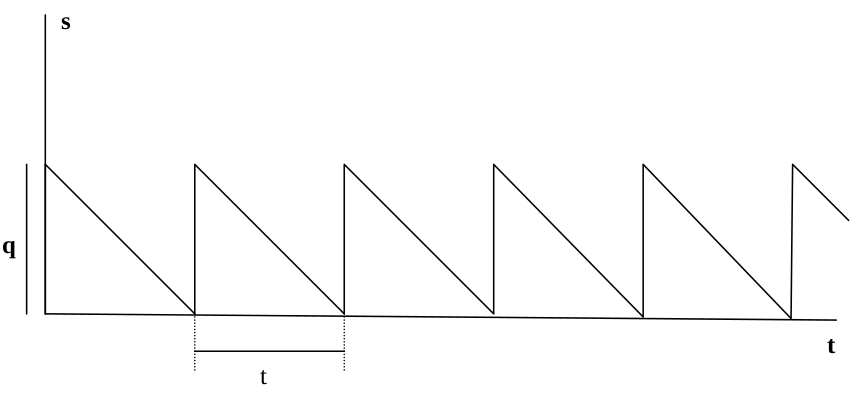
\includegraphics[width=\linewidth]{imagenes/stock-modelo-basico.png}
\end{figure}

Para un ciclo cualquiere \(i\), el \textbf{costo total de adquisición} será:

\[
    b.q
\]

El costo total de almacenamiento para un ciclo, es el area bajo la curva.

\[
    \frac{1}{2} \cdot q \cdot c_1 \cdot t
\]
Por ultimo el \textbf{costo total de orden} es siplemente \(k\) porque se emite un solo pedido por ciclo. 
Por lo tanto, el \textbf{costo total esperado} por ciclo es:

\begin{equation}
    CTE_i= b \cdot q+\frac{1}{2} \cdot q \cdot c_1 \cdot t + k
\end{equation}

El número de ciclos por periodo de referencia (ej: un año) es el cosiente entre la \textbf{demanda anual} \(D\) 
y la cantidad solicitada en cada ciclo \(q\); o también el cociente entre el parametro \(T\) (equivale a 1) y \(t\)
(duración de un ciclo, expresada en unidad de año).

\begin{equation}
    n=\frac{D}{q}=\frac{T}{t}
\end{equation}


Luego, multiplicamos \(CTE_i\) y \(n\), obtenemos el \textbf{costo total esperado anual}:


\begin{equation}
    CTE= b \cdot D +\frac{1}{2} \cdot q \cdot c_1 \cdot T + k \cdot \frac{D}{q}
\end{equation}


Esta última función es la que necesitamos minimizar siendo \(q\) la variable a derivar y 
luego igualando a cero.

\begin{figure}[h!]
    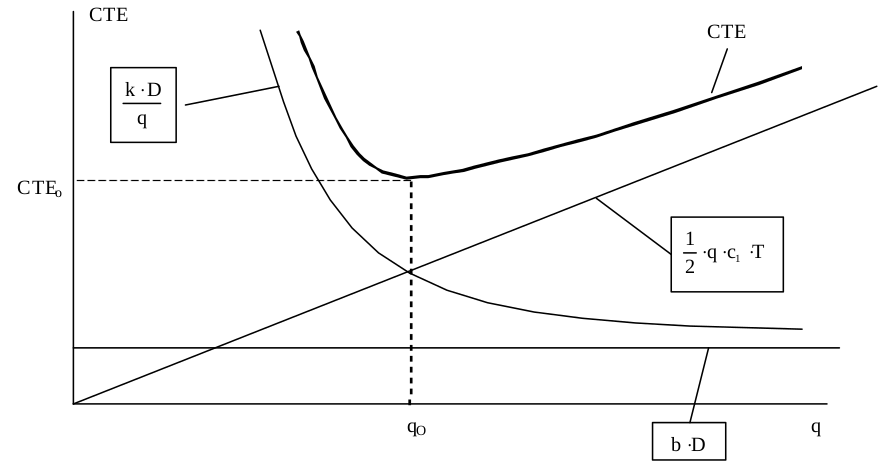
\includegraphics[width=\linewidth]{imagenes/stock-q-optimo.png}
\end{figure}

\[
    \frac{\partial CTE}{ \partial q} = \frac{1}{2} \cdot c_1 \cdot T - k \cdot \frac{D}{q^2} = 0
\]

Como la derivada segunda es positiva, tendremos un minimo en ese punto. Despejando \(q_o\):

\begin{equation}
    q_o = \sqrt{\frac{2 \cdot k \cdot D}{T \cdot c_1}}
\end{equation}
Este es el tamaño de lote óptimo.

Luego, hallamos el \textbf{Costo Total Esperado} óptimo, reemplazando \(q_o\) en \(CTE\):

\begin{equation}
    CTE_o = b \cdot D + \sqrt{2 \cdot k \cdot D \cdot T \cdot c_1}
\end{equation}

A partir de la formula de \(n\), obtenemos a \(t_o\) y a \(n_o\):

\begin{equation}
    t_o = \sqrt{\frac{2 \cdot k \cdot T}{D \cdot c_1}}
\end{equation}

\begin{equation}
    n_o = \sqrt{\frac{T \cdot c_1 \cdot D}{2 \cdot k}}
\end{equation}

Tambien se puede determinar el \textbf{stock de reorden} o punto de pedido, en base al \textit{lead time} y la \textit{tasa de demanda} \(d\):

\begin{equation}
    S_R = LT \cdot d
\end{equation}

\begin{figure}[h!]
    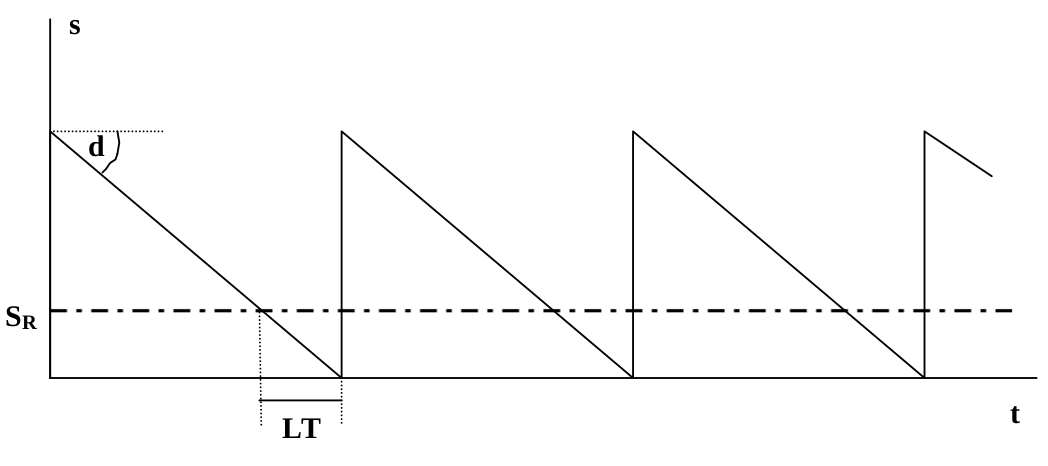
\includegraphics[width=\linewidth]{imagenes/stock-reorden.png}
\end{figure}


\newpage
\subsection{Restricciones}

Ahora si plenteamos distintas variantes de restricciones que puede haber a partir de este modelo:

\begin{itemize}
    \item Fisicas
    \item Administrativas.
    \item Financieras:
    \item Operativas
    \item Condiciones de la variable.
\end{itemize}

\subsubsection{Restricciones Fisicas}

Definimos:
\begin{itemize}
    \item SU: Superficie ocupada por cada unidad de producto.
    \item SUPTOT: Superficie total disponible.
\end{itemize}
Se debe cumplir la resticción \(SUP \cdot q \leq SUPTOT\) despues de calcular el \(q_o\). 
Si no se cumple se debe calcular el nuevo lote de compra \(q*\) que no sera el óptimo:

\begin{equation}
    q* = \frac{SUBTOT}{SU}
\end{equation}


\subsubsection{Restricciones Financieras}
Existe una restricción de capital máximo a inmovilizar. Entonces definimos, \(CMI\) como el capital máximo a inmovilizar,
y se debe cumplir la restricción \(b \cdot q \leq CMI\), utilizando el \(q_o\).

Si no se cumple la restricción, se debe calcular el nuevo lote de compra \(q*\) que no sera el óptimo:

\begin{equation}
    q* = \frac{CMI}{b}
\end{equation}

\subsubsection{Restricciones Administrativas}
Existe una cantidad de ordenes a emitir. Se defino \(CMO\) como la cantidad máxima de ordenes a emitir y 
se debe cumplir la restricción \(\frac{D}{q} \leq CMO\), utilizando el \(q_o\).

Si no se cumple la restricción, se debe calcular el nuevo lote de compra \(q*\) que no sera el óptimo:

\begin{equation}
    q* = \frac{D}{CMO}
\end{equation}

Notar que si se quiere hallar CTE no se debe utilizar la formula de \(CTE_o\), sino que se debe partir de la formula general
remplando \(q\) por \(q*=\frac{D}{CMO}\).

\subsubsection{Restricciones de condiciones de variable}

Si se impone como restricción que el \textit{stock debe ser cero} al finalizar el periodo de estudio,
Entonces la restricción es que la \textbf{cantidad de ciclos debe ser entero}.

Si al calcular \(n_o = \frac{D}{q_o}\) no cumple la restricción, se debe calcular los \(CTE\) (con la formula sin derivar) para los valores
de q para dos valores enteros de \(n\) entre los valores de \(n_o\) y nos quedamos que el \(n\) con menor costo total esperado (CTE).







\newpage
\subsection{Modelo básico con protección de stock}

El \textbf{Stock de Protección} es un nivel de existencias que se mantiene a los fines de absorber situaciones imprevistas.
Se utiliza en los siguientes casos:

\begin{itemize}
    \item Absorber aleatoriedad de la demanda.
    \item Tiempo de aprovisionamiento cuando la demanda es aleatoria.
    \item Cuando el costos de agotamiento es muy alto(ejemplo: Materias primas).
    \item Cuando se quiere mantener un excelente nivel de servicio.
\end{itemize}

\noindent
\underline{HIPOTESIS:}
\begin{enumerate}
    \item Se administra un único ítem.
    \item El producto es de demanda independiente.
    \item La demanda es conocida y se efectúa a tasa constante.
    \item El plazo de entrega ("lead time") del producto solicitado, es conocido y constante.
    \item \textbf{Se mantiene un stock de seguridad. Es stock que no se utiliza operativamente}.
    \item El aprovisionamiento es instantaneo. Tasa de reposición es infinita.
    \item El horizonte de planeamiento es de largo plazo.
    \item \textbf{No se admite agotamiento.}
    \item El costo de adquisición "b", cost. uni. de almacenamiento "\(c_1\)" y el costo de pedido "k" son independientes de la cantidad a pedir "q".
    \item No hay restricciones sobre el tamaño a tomar del lote.
    \item Todos los parametros monetarios estan expresados en moneda constante.
    \item El producto se mide en una unidad continua. (Litros, kilogramos, etc).
\end{enumerate}


\noindent
\underline{PARAMETROS:}
\begin{itemize}
    \item Idem parametro de modelo básico.
    \item \(S_P\): Stock de protección
\end{itemize}


\noindent
\underline{VARIABLES:}
\begin{itemize}
    \item Idem variables de modelo básico.
    \item S: Stock máximo.
\end{itemize}


\underline{Modelado}


\begin{figure}[h!]
    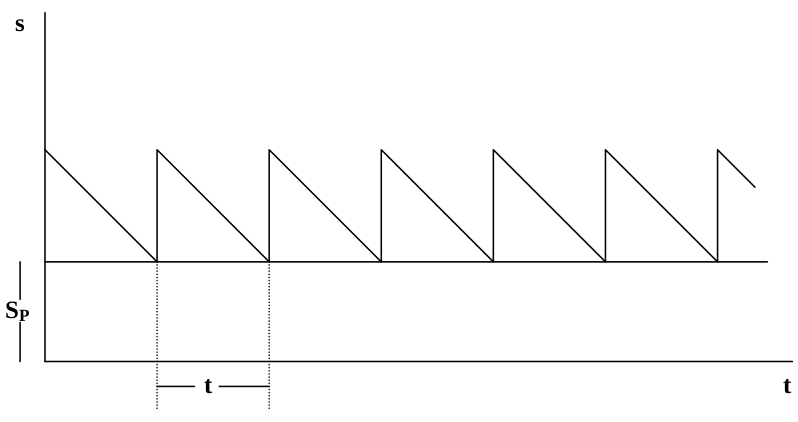
\includegraphics[width=0.8\textwidth]{imagenes/stock-proteccion.png}
\end{figure}

Para un ciclo cualquiera, tendremos la siguiente expresión del costo total esperado:

\begin{equation}
    CTE_i= b \cdot q+\frac{1}{2} \cdot q \cdot c_1 \cdot t + k + S_P \cdot c_1 \cdot t
\end{equation}

Multiplicando por \(n\) obtenemos:

\begin{equation}
    CTE= b \cdot D +\frac{1}{2} \cdot q \cdot c_1 \cdot T + k \cdot \frac{D}{q} + S_P \cdot c_1 \cdot T
\end{equation}

Obtenemos el valor optimo de \(q\), el cual es independiente del nivel de stock de protección:

\begin{equation}
    q_o = \sqrt{\frac{2 \cdot k \cdot D}{T \cdot c_1}}
\end{equation}

Obtenemos el \textbf{costo total esperado} con stock de protección:

\begin{equation}
    CTE_o = b \cdot D + \sqrt{2 \cdot k \cdot D \cdot T \cdot c_1} + S_P \cdot C_1 \cdot T
\end{equation}

Tambien hallamos \(t_o\) y \(n_o\)

\begin{equation}
    t_o = \sqrt{\frac{2 \cdot k \cdot T}{D \cdot c_1}}
\end{equation}

\begin{equation}
    n_o = \sqrt{\frac{T \cdot c_1 \cdot D}{2 \cdot k}}
\end{equation}

Luego, al \textbf{stock de reorden} se suma el stock de protección:

\begin{equation}
    S_R = LT \cdot d + S_P
\end{equation}

El \textbf{stock maximo de almacen} es la suma de \(q_o\) y el stock de protección:

\begin{equation}
    S = q_o + S_P
\end{equation}

En conclución el \textbf{stock de protección} no impacta en el tamaño del lote \(q\), pero si impacta en el punto de 
pedido \(S_R\) o punto de reorden. Sobre el stock de protección se pueden montar otros modelos. 





\newpage
\subsection{Modelo básico con agotamiento admitido}

El agotamiento de las existencias se verifica cuando no quedan más unidades disponibles para satisfacer la demanda.

\noindent
\underline{HIPOTESIS:}
\begin{enumerate}
    \item Se administra un único ítem.
    \item El producto es de demanda independiente.
    \item La demanda es conocida y se efectúa a tasa constante.
    \item El plazo de entrega ("lead time") del producto solicitado, es conocido y constante.
    \item La reposición se hace exactamente cuando el nivel de stock es cero.
    \item \textbf{El agotamiento esta permitido}. 
    \item El horizonte de planeamiento es de largo plazo.
    \item El costo de adquisición "b", cost. uni. de almacenamiento "\(c_1\)" y el costo de pedido "k" son independientes de la cantidad a pedir "q".
    \item No hay restricciones sobre el tamaño a tomar del lote.
    \item Todos los parametros monetarios estan expresados en moneda constante.
    \item El producto se mide en una unidad continua. (Litros, kilogramos, etc).
    \item \textbf{El costo de agotamiento esta dado por el costo en el que se incurre por unidad de tiempo de deficit.}
\end{enumerate}

\noindent
\underline{PARAMETROS:}
\begin{itemize}
    \item Idem parametro de modelo básico.
    \item \(c_2[\$/u.t]\): Costo de agotamiento por unidad de tiempo de postergarción.
\end{itemize}

\noindent
\underline{VARIABLES:}
\begin{itemize}
    \item Idem variables de modelo básico.
    \item \(t_1\): Periodo de entrega de mercadería.
    \item \(t_2\): Periodo de déficit de mercadería.
    \item \(S_A\): Cantidad máxima de unidades agotadas.
\end{itemize}


\newpage
\underline{MODELADO:}

\begin{figure}[h!]
    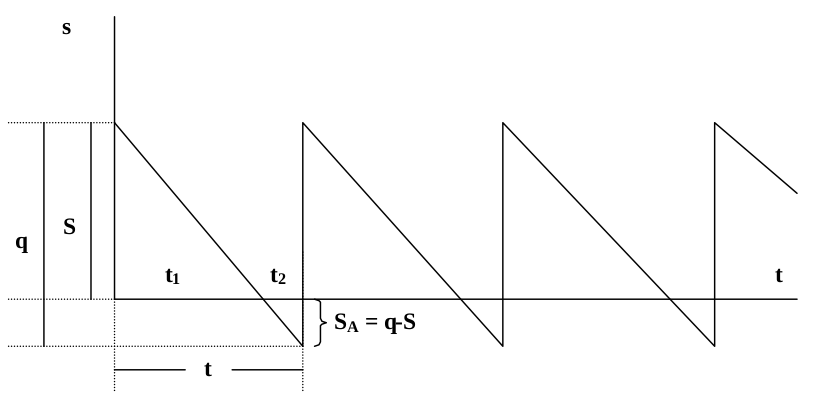
\includegraphics[width=0.8\textwidth]{imagenes/stock-modelo-agotamiento.png}
\end{figure}

El costo total esperado por ciclo sera:

\begin{equation}
    CTE_i= b \cdot q + \frac{1}{2} \cdot S \cdot c_1 \cdot t_1 + \frac{1}{2} \cdot (q - S) \cdot c_2 \cdot t_2 + k
\end{equation}

Pero, como se calculan \(t_1\)y \(t_2\), utilizando relación entre triangulos:

\begin{equation}
    \frac{S}{q} = \frac{t_1}{t_i}  \implies t_1 = t_i \cdot \frac{S}{q}
\end{equation}

\begin{equation}
    \frac{q-S}{q} = \frac{t_2}{t_i}  \implies t_2 = t_i \cdot \frac{q-S}{q}
\end{equation}

La expresión de \textbf{lote optimo de adquisición} es:

\begin{equation}
    q_o = \sqrt{\frac{2 \cdot k \cdot D}{T \cdot c_1}} \cdot \sqrt{\frac{c_1+c_2}{c_2}}
\end{equation}

La expresión del valor óptimo de la \textbf{cantidad máxima a almacenar} \(S\):

\begin{equation}
    S_o = \sqrt{\frac{2 \cdot k \cdot D}{T \cdot c_1}} \cdot \sqrt{\frac{c_2}{c_1+c_2}}
\end{equation}

\begin{equation}
    S_o = \frac{q_o \cdot c_2}{c_1 + c_2}
\end{equation}

La expresión para la \textbf{cantidad máxima agotada óptima} por período:

\begin{equation}
    S_{Ao} = q_o \cdot \frac{c_1}{c_1 + c_2}
\end{equation}


\begin{equation}
    S_{Ao} = q_o - S_o
\end{equation}

Luego, hallamos el \textbf{Costo Total Esperado} óptimo, sera:

\begin{equation}
    CTE_o = b \cdot D + \sqrt{2 \cdot k \cdot D \cdot T \cdot c_1} \cdot \sqrt{\frac{c_2}{c_1 + c_2}}
\end{equation}


Intervalo óptimo de cada ciclo:

\begin{equation}
    t_o = \frac{q_o \cdot T}{D}
\end{equation}

Periodo óptimo de entrega:

\begin{equation}
    t_{1o} = t_{io} \cdot \frac{S_o}{q_o}
\end{equation}

Periodo óptimo de déficit:

\begin{equation}
    t_{2o} = t_{io} \cdot \frac{q_o - S_o}{q_o}
\end{equation}

Número óptimo de pedidos a efectuar:

\begin{equation}
    n_o = \frac{D}{q_o}
\end{equation}


\newpage
\begin{figure}[h!]
    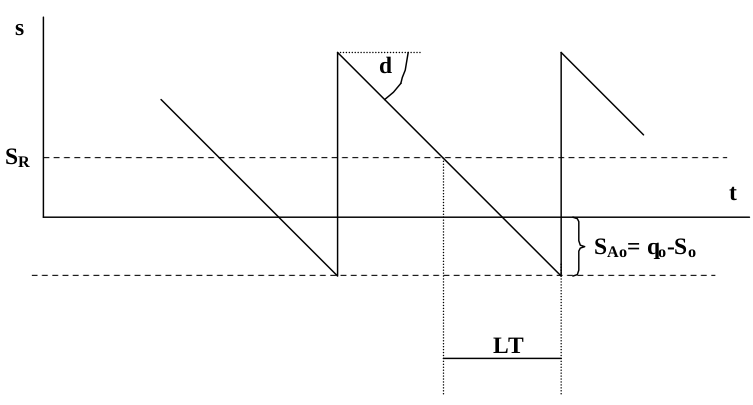
\includegraphics[width=\linewidth]{imagenes/stock-reorden-agotamiento.png}
\end{figure}

Finalmente, obtendremos el stock de reorden de:

\begin{equation}
    S_R = LT \cdot d - S_{Ao}
\end{equation}


\newpage
\subsection{Modelo Reposición no instantaneo}

El ingreso de producto al almacen no es instantanea y se realiza a tasa constante.


\noindent
\underline{HIPOTESIS:}
\begin{enumerate}
    \item Se administra un único ítem.
    \item El producto es de demanda independiente.
    \item La demanda es conocida y se efectúa a tasa constante.
    \item El plazo de entrega ("lead time") del producto solicitado, es conocido y constante.
    \item La reposición no es instantaneo. La tasa de aprovisionamiento es finita.
    \item El horizonte de planeamiento es de largo plazo.
    \item El costo de agotamiento es infinitamente alto. El agotamiento no está permitido.
    \item El costo de adquisición "b", cost. uni. de almacenamiento "\(c_1\)" y el costo de pedido "k" son independientes de la cantidad a pedir "q".
    \item No hay restricciones sobre el tamaño a tomar del lote.
    \item Todos los parametros monetarios estan expresados en moneda constante.
    \item El producto se mide en una unidad continua. (Litros, kilogramos, etc).
\end{enumerate}


\noindent
\underline{PARAMETROS:}
\begin{itemize}
    \item Idem parametro de modelo básico.
    \item \(P[u/t]\): Reposición del producto a un periodo t. 
    \item \(p[u/t]\): Tasa de reposición
\end{itemize}

\noindent
\underline{VARIABLES:}
\begin{itemize}
    \item Idem variables de modelo básico.
    \item \(t_1\): Periodo de aprovisionamiento.
    \item \(t_2\): No hay ingreso de mercaderia. Solo hay egresos.
\end{itemize}

\noindent
\underline{MODELADO:}

\begin{figure}[h!]
    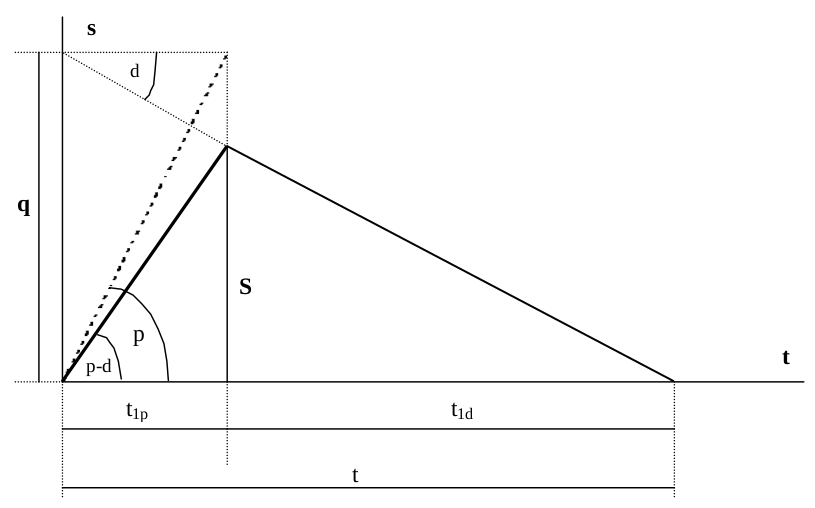
\includegraphics[width=\linewidth]{imagenes/stock-modelo-no-instantaneo.png}
\end{figure}

Determinar el \(CTE\) en cada ciclo \(i\):
\begin{equation}
    CTE_i= b \cdot q + \frac{1}{2} \cdot S \cdot c_1 \cdot t + k
\end{equation}

Del grafico se puede obtener \(S\) y \(t_1\):

\begin{equation}
    q= p \cdot t_1 \implies t_1 = \frac{q}{p}
\end{equation}

\begin{equation}
    S = q \cdot (1 - \frac{d}{p})
\end{equation}

Remplazando S, entonces el costo esperado total para los \(n\) ciclos sera(la ecuación a minimizar):

\begin{equation}
    CTE = b \cdot D + \frac{1}{2} \cdot q \cdot (1-\frac{d}{p}) \cdot c_1 \cdot T + \frac{k \cdot D}{q} 
\end{equation}

Derivando y despejando, obtenemos el \(q_o\):

\begin{equation}
    q_o = \sqrt{\frac{2 \cdot k \cdot D}{T \cdot c_1 \cdot (1-\frac{d}{p})}}
\end{equation}

Reemplazando el \(q_o\), obtenemos el \(CTE_o\) óptimo:

\begin{equation}
    CTE_o = b \cdot D + \sqrt{2 \cdot k \cdot D \cdot T \cdot c_1 \cdot (1-\frac{d}{p})}
\end{equation}

El tamaño de  stock maximo sera:

\begin{equation}
    S_o = q_o \cdot (1-\frac{d}{p})
\end{equation}

Seguimos y hallamos \(t_o\); \(t_1\); \(t_2\) y \(n_o\):

\begin{equation}
    t_o = \frac{T}{D} \cdot q_o = \sqrt{\frac{2 \cdot k \cdot T}{D \cdot c_1 \cdot (1-\frac{d}{p})}}
\end{equation}


\begin{equation}
    t_1 = \frac{q_o}{p} = \sqrt{\frac{2 \cdot k \cdot T}{D \cdot c_1 \cdot (1-\frac{d}{p})}}
\end{equation}

\begin{equation}
    n_o = \frac{D}{q_o} = \sqrt{\frac{T \cdot c_1 \cdot (1-\frac{d}{p}) \cdot D }{2 \cdot k}}
\end{equation}

Para determinar el \textbf{stock de reorden}: 

\begin{itemize}
    \item Si \( LT \leq t-t_1 \implies S_R = LT \cdot d \)
    \item Si \( LT > t-t_1 \implies S_R = (t-LT) \cdot (p-d)\)    
\end{itemize}


\subsection{Modelo Reaprovicionamiento Constantes - Descarga instantanea}

\subsubsection{Hipotesis}
\begin{itemize}
    \item Se admite un unico item.
    \item La producción es conocida y se efectúa a tasa constante
    \item La demanda se satisface con la descarga del producto por medio de lotes, a intervalos regulares de tiempo.
    \item El lead time es conocido y constante.
    \item No hay stock de protección.
    \item \textbf{La descarga es instantanea}.
    \item El horizonte de planeamiento es a largo plazo.
    \item No se admite deficit del producto.
    \item El costo de adquisición "b", cost. uni. de almacenamiento "\(c_1\)" y el costo de pedido "k" son independientes de la cantidad a pedir "q".
    \item No hay restricciones sobre el tamaño a tomar del lote.
    \item Todos los parametros monetarios estan expresados en moneda constante.
    \item El producto se mide en una unidad continua. (Litros, kilogramos, etc).
\end{itemize}

\noindent
\underline{PARAMETROS:}
\begin{itemize}
    \item Idem parametro de modelo básico.
    \item \(P[u/t]\): Producción del producto a un periodo t. \(P=D\) en todo el periodo.
    \item \(p[u/t]\): Tasa de producción
\end{itemize}

\noindent
\underline{VARIABLES:}
\begin{itemize}
    \item Idem variables de modelo básico.
\end{itemize}


\noindent
\underline{MODELADO:}

\begin{figure}[h!]
    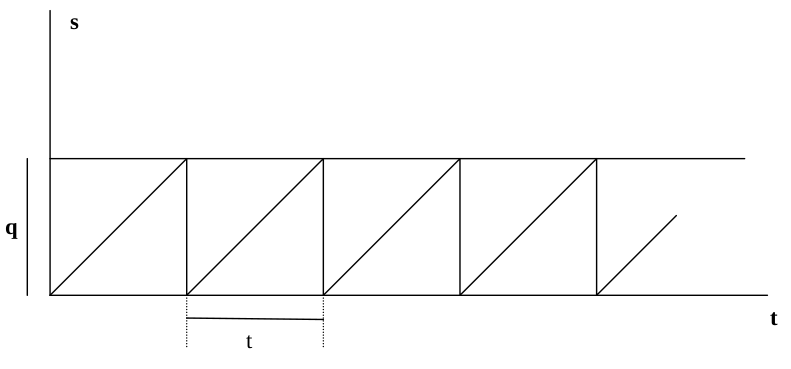
\includegraphics[width=\linewidth]{imagenes/modelo-stock-aprovicionamiento-constante.png}
\end{figure}
Determinar el \(CTE\) en cada ciclo \(i\):
\begin{equation}
    CTE_i= b \cdot q + \frac{1}{2} \cdot S \cdot c_1 \cdot t + k
\end{equation}

Del grafico se puede obtener el numero de ciclos como:

\begin{equation}
    n = \frac{P}{q} = \frac{T}{t}
\end{equation}

Luego el \(CTE\) anual será:
\begin{equation}
    CTE = b \cdot P + \frac{1}{2} \cdot q \cdot c_1 \cdot T + k \cdot \frac{P}{q}
\end{equation}

Derivando con respecto a "q" e igualando a cero se obtiene la expresión del lote total de descarga (fórmula de Wilson) :

\begin{equation}
    q_o = \sqrt{\frac{2 \cdot k \cdot P}{T \cdot c_1 }}
\end{equation}

Reemplazando el \(q_o\), obtenemos el \(CTE_o\) óptimo:

\begin{equation}
    CTE_o = b \cdot D + \sqrt{2 \cdot k \cdot P \cdot T \cdot c_1 }
\end{equation}

Finalmente, conocido el plazo de descarga (LT), se podrá determinar el stock de reorden 
mediante la siguiente expresión:

\begin{equation}
    S_r = q_o - LT \cdot p
\end{equation}




\end{document}
